\chapter{Принцип возможных перемещений (принцип Лагранжа). Доказательство
необходимости и достаточности. Примеры применения принципа возможных
перемещений.}

\section{Принцип возможных перемещений}
Для того, чтобы система материальных точек, подчиненная идеальным стационарным и
удерживающим связям, находилась в равновесии, необходимо и достаточно, чтобы
работа всех активных сил на любом виртуальном перемещении системы и скорости
всех точек в начальный момент времени равнялись нулю. Таким образом, нужно
доказать, что необходимо и достаточно выполнение условий:
\[
    \sum_{k=1}^N \vec{F}_k\cdot\delta\vec{r}_k = 0,\quad
    \vec{v}_k(0) = 0 \quad (k = 1, 2, \ldots, N).
\]

\emph{Необходимость.} Пусть система находится в равновесии, тогда должны
выполняться условия: \( \vec{F}_k + \vec{R}_k = 0,\ \vec{v}_k(0) = 0 \).

Пусть система совершила виртуальное перемещение \( \delta\vec{r}_1 \), \ldots,
\( \delta\vec{r}_n \). Умножим каждое уравнение равновесия на
\( \delta\vec{r}_k \) и просуммируем: \( \ds \sum_{k=1}^n \vec{F}_k\cdot\delta
\vec{r}_k + \sum_{k=1}^n \vec{R}_k\cdot\delta\vec{r}_k = 0 \).
 
Так как связи идеальны, то последняя сумма равна нулю. Следовательно, при
равновесии системы выполняется равенство: \( \ds \sum_{k=1}^n \vec{F}_k\cdot
\delta\vec{r}_k = 0 \), доказывающее необходимость.

\emph{Достаточность.} Для доказательства достаточности нужно показать, что при
выполнении условий система будет находиться в равновесии. Применим теорему об
изменении кинетической энергии. Предположим, что условия выполнены, но система
под действием приложенных сил начала двигаться. По условию теоремы все связи
стационарны, поэтому перемещение системы за время \( dt \) будет совпадать с
одним из виртуальных перемещений \( \delta\vec{r}_1, \ldots, \delta\vec{r}_n \).
На основе теоремы об изменении кинетической энергии сумма работ всех активных
сил и реакций связей на этом перемещении будет положительна, тогда:
\( \ds \sum_{k=1}^n \vec{F}_k\cdot\delta\vec{r}_k + \sum_{k=1}^n \vec{R}_k\cdot
\delta\vec{r}_k > 0 \). По условию теоремы связи идеальны, поэтому второе
слагаемое равно нулю. Следовательно,
\( \ds \sum_{k=1}^n \vec{F}_k\cdot\delta\vec{r}_k > 0 \).

Несовместимость этого неравенства с принятым предложением доказывает
достаточность условий принципа виртуальных перемещений.

\begin{minipage}{.4\textwidth}
    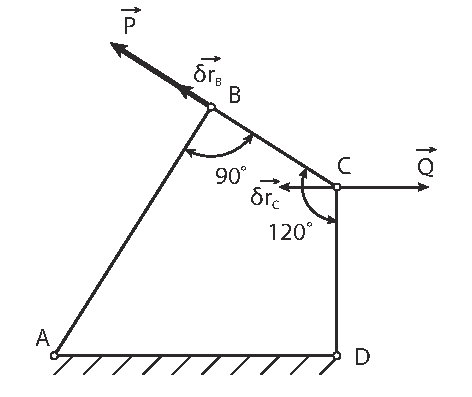
\includegraphics[width=\textwidth]{28_01}
\end{minipage}
\begin{minipage}{.55\textwidth}
\section{Пример}
К шарнирам \( B \) и \( C \) четырехзвенника \( ABCD \) приложены две силы
\( \vec{P} \) и \( \vec{Q} \), перпендикулярные звеньям \( AB \) и \( CD \)
соответственно. Считая силу \( \vec{P} \) известной, определить силу
\( \vec{Q} \) при равновесии системы, если \( \angle ABC = 90^\circ \), а
\( \angle BCD = 120^\circ \). Массами пренебречь.

\emph{Решение.} Дадим системе виртуальное перемещение. Так как стержень \( AB \)
может вращаться вокруг оси \( A \), а стержень \( CD \) -- вокруг оси \( D \),
то виртуальное перемещение \( \delta\vec{r}_B \) точки \( B \)
\end{minipage}
перпендикулярно \( AB \), а виртуальное перемещение \( \delta\vec{r}_C \) точки
\( C \) перпендикулярно \( CD \). Применяя принцип возможных перемещений,
получим: \( \vec{P}\cdot|\delta\vec{r}_B| - \vec{Q}\cdot|\delta\vec{r}_C| = 0\).

Учтем, что проекции виртуальных перемещений двух точек твердого тела на прямую,
соединяющую эти точки, равны между собой. Для точек \( B \) и \( C \) имеем:
\( |\delta r_B| = |\delta r_C|\cos 30^\circ \).

Подставляя это в предыдущие равенство, получим:
\( P\cdot|\delta r_C|\cos 30^\circ - Q\cdot|\delta r_C| = 0 \), откуда
\[
    Q = P\cos 30^\circ = P\cdot\sqrt{3}/2.
\]

\newpage % ---------------------------------------------------------------------
